\section{Exercícios}

\begin{exercise}
    Formam-se $n$ triângulos com palitos, conforme a figura abaixo.
\begin{center}

\begin{figure}[H]
    \center
    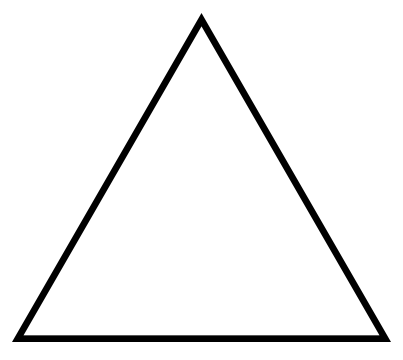
\includegraphics[width=1.5cm]{../../../res/img/fig-c05-exrPalitos-01.png}
    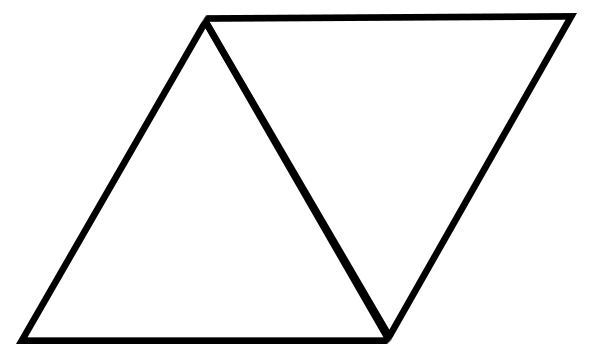
\includegraphics[width=2.15cm]{../../../res/img/fig-c05-exrPalitos-02.png}
    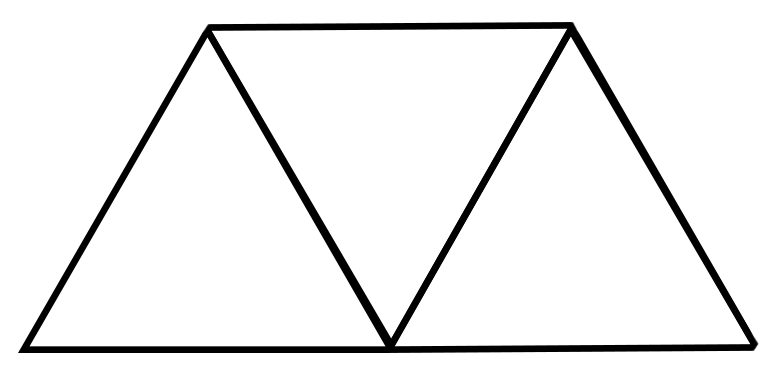
\includegraphics[width=2.8cm]{../../../res/img/fig-c05-exrPalitos-03.png}
    %TODO: captions (\textbf{$n=1$}, 2, 3)
\end{figure}

\end{center}
Qual o número de palitos usados para construir $n$ triângulos? 
\end{exercise}

\begin{exercise}
    A soma dos ângulos internos de um pentágono convexo é igual a
540\tdeg e estes ângulos estão em PA. Determine a mediana dos valores
dos ângulos.
\end{exercise}

\begin{exercise}
    Se $3-x$, $-x$, $\sqrt{9-x}$, $\dots$ é uma PA, determine $x$ e
calcule o quinto termo.
\end{exercise}

\begin{exercise}
    Calcule a soma dos termos da PA 2, 5, 8, 11, $\dots$ desde o 25\tdeg
termo até o 41\tdeg termo, inclusive.
\end{exercise}

\begin{exercise}
    Determine o maior valor inteiro que pode ter a razão de uma PA
que admita os números 32, 227 e 942 como termos da progressão.
\end{exercise}

\begin{exercise}
    O gordinho jaguatirica e Júnio vão jogar um  jogo com as
seguintes regras:
\begin{itemize}
  \item Na primeira jogada, o gordinho jaguatirica escolhe um número no
  conjunto $A = \set{1, 2, 3, 4, 5, 6, 7}$ e diz esse número;
  \item Os jogadores jogam alternadamente;
  \item Cada jogador ao jogar escolhe um elemento de $A$, soma-o ao
  número DITO pelo jogador anterior e DIZ a soma;
  \item O vencedor é aquele que disser 63.
\end{itemize}
Pode o gordinho jaguatirica ou Júnio ter uma estratégia vencedora?
Se sim, quem pode e qual é essa estratégia?
\end{exercise}

%\Ex{Refaça o exercício anterior para o caso do vencedor ser quem
%disser 64.}

%\Ex{Refaça o penúltimo exercício para o caso de $A = \set{3, 4, 5,
%6}$.}

\begin{exercise}
    Mostre que Júnio pode ter uma estratégia que impeça o gordinho
vencer o jogo se a condição de vitória for 62 e $A =\set{3, 4, 5, 6,
7}$. 
\end{exercise}

\begin{exercise}
    Em um quadrado mágico (Exemplo \ref{ex:quadrado-magico-3x3}),
chamamos de constante mágica o valor da soma de quaisquer uma das
linhas, colunas ou diagonais. Calcule a constante mágica de um
quadrado mágico $n \times n$.
\end{exercise}

\begin{exercise}
    Calcule a soma de todos os inteiros que divididos por $11$ dão resto $7$ e estão compreendidos entre $200$ e $400$.
\end{exercise}
%\Ex{Podem os números $\sqrt 2$, $\sqrt 3$ e $\sqrt 5 $ pertencer a
%uma mesma PA?}


\begin{exercise}
Suprimindo um dos elementos do conjunto $\set{1, 2, \dots , n}$,
a média aritmética dos elementos restantes é $16{,}1$. Determine o
valor de $n$ e qual foi o elemento suprimido.    
\end{exercise}

%\Ex{Um bem, cujo valor hoje é de R\$ 8000,00, desvaloriza-se de tal
%forma que seu valor daqui a 4 anos será de R\$ 2000,00. Supondo
%constante a desvalorização anual, qual será o valor do bem daqui a 3
%anos? }

\begin{exercise}
    Descontos sucessivos de 10\% e 20\% equivalem a um desconto
total de quanto?
\end{exercise}

%\Ex{Um aumento de 10\% seguido de um desconto de 20\% equivale a um
%desconto único de quanto?}

%\Ex{Aumentando sua velocidade em 60\%, de quanto você diminui o
%tempo de viagem?}

\begin{exercise}
    Um decrescimento mensal de 5\% gera um decrescimento anual de
quanto?
\end{exercise}

%\Ex{O período de um pêndulo simples é diretamente proporcional à
%raiz quadrada do seu comprimento. De quanto devemos aumentar o
%comprimento para aumentar o período em 20\%?}

\begin{exercise}
    Mantida constante a temperatura, a pressão de um gás perfeito é
inversamente proporcional a seu volume. De quanto aumenta a pressão
quando reduzimos em 20\% o volume?
\end{exercise}

%\Ex{Se a base de um retângulo aumenta em 10\% e a altura diminui em
%10\%, quanto aumenta a sua área?}

%\Ex{Um carro novo custa R\$ 18000,00 e, com 4 anos de uso, vale R\$
%12000,00. Supondo que o valor decresça a uma taxa anual constante,
%determine quanto vale o carro com 1 ano de uso.}

\begin{exercise}
    Considere um triângulo retângulo tal que seus lados formam uma
PG crescente. Determine a razão dessa progressão.
\end{exercise}

\begin{exercise}
    Qual o quarto termo da PG $\sqrt 2 , \sqrt[3] 2 , \sqrt[6] 2 ,
\dots$?
\end{exercise}

\begin{exercise}
    Determine três números em PG, tais que a soma desses números é
19 e a soma de seus quadrados é 133.
\end{exercise}

\begin{exercise}
    A soma de três números em PG é 19. Subtraindo-se 1 do primeiro,
eles passam a formar uma PA. Calcule-os.
\end{exercise}

\begin{exercise}
    Quatro números que estão em sequência são tais que, os três
primeiros formam uma PA de razão 6, os três últimos uma PG e o
primeiro número é igual ao quarto. Determine-os.
\end{exercise}

\begin{exercise}
Será formada uma pilha de folhas de estanho que têm, cada uma,
espessura de $0,1$mm. Inicialmente, adiciona-se uma folha na pilha.
Nas operações seguintes, é inserida uma quantidade de folhas igual
ao número de folhas que já estavam na pilha no momento da inserção.
Após serem realizadas 33 adições de folhas, a altura da pilha será,
aproximadamente:
\begin{enumerate}[a.]
  \item A altura de um poste de luz;
  \item A altura de um prédio de 40 andares;
  \item O comprimento da praia de Copacabana;
  \item A distância Rio-São Paulo;
  \item O comprimento do equador terrestre.
\end{enumerate}
\end{exercise}

\begin{exercise}
    Começando com um segmento de tamanho 1, divide-se esse segmento em três partes iguais e retiramos o segmento da parte central, obtendo dois segmentos de comprimento $\dfrac 1 3$. Repetimos essa operação com cada um desses segmentos e assim por diante.
    \begin{figure}[H]
        \centering
        \label{fig:exercicio-segmento}
        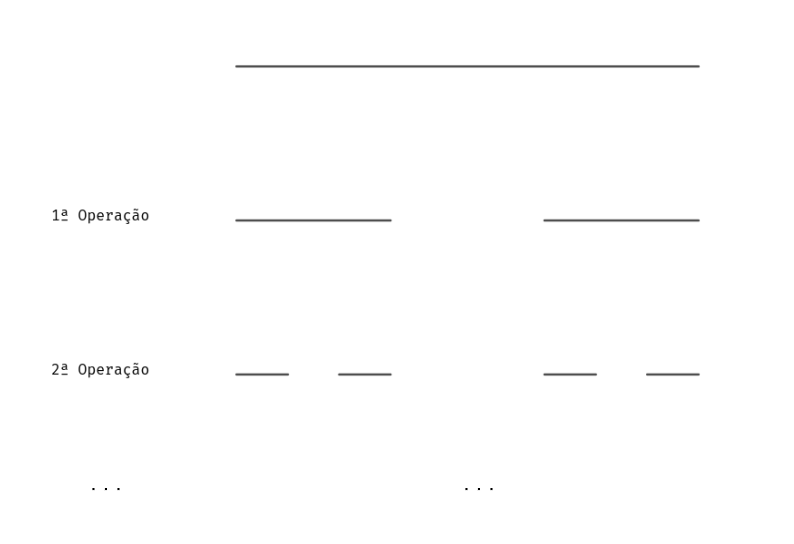
\includegraphics[width=15cm]{\imgdirfromsection/exercicio-segmento.png}
	\caption{Operações no segmento.}
    \end{figure}
    \begin{enumerate}[a)]
	\item Determine o termo geral da progressão dos comprimentos dos segmentos em cada uma dessas operações;
	\item Determine a soma $S_n$ dos comprimentos dos segmentos até a $n$-ésima operação.
    \end{enumerate}
\end{exercise}

\begin{exercise}
    Larga-se uma bola de uma altura de 5m. Após cada choque com o
solo, ela recupera apenas $\frac 4 9 $ da altura anterior. 
%
\begin{enumerate}[a.]
    \item Determine a progressão que modela o problema e calcule 
    a altura que a bola atinge após o décimo choque com o solo
    e após o centésimo choque com o solo.
    \item Qual a distância total percorrida pela bola no momento 
    do décimo primeiro choque com o solo? 
\end{enumerate}
\end{exercise}

\begin{exercise}
	Demonstre, por indução, a fórmula do somatório dos $n$ primeiros termos de uma PA:
	\[S_n = \frac {\prn {a_1+a_n}n} 2.\]
\end{exercise}

\begin{exercise}
	Demonstre, por indução, a fórmula do somatório dos $n$ primeiros termos de uma PG:
	\[S_n = a_1 \cdot \frac{1-q^n}{1-q}.\]
\end{exercise}

\begin{exercise}
   Dizemos que dois triângulos $ABC$ e $DEF$ são \emph{semelhantes} quando há uma correspondência entre seus vértices de tal modo que a razão do comprimento de seus lados correspondentes é constante, ou seja,
   $$ \dfrac{\overline{AB}}{\overline{DE}} = \dfrac{\overline{AC}}{\overline{DF}} = \dfrac{\overline{BC}}{\overline{EF}}.$$

    Na figura abaixo, temos uma poligonal onde os segmentos alternam entre ser perpendicular a $AB$ e ser perpendicular a $AC$, formando triângulos semelhantes. O comprimento do primeiro segmento é $a$ e o do segundo é $b$.
    \begin{figure}[H]
	\centering
	\importtikz{exercicio-poligonal}
        \caption{Poligonal}
        \label{fig:my_label}
    \end{figure}
\end{exercise}

\begin{exercise}\label{ex:espiral}
    Uma espiral é formada por semicírculos em torno do eixo $x$ conforme ilustra a imagem abaixo. O primeiro semicírculo liga a origem ao ponto $(a_1, 0)$, o segundo semicírculo liga o ponto $(a_1, 0)$ ao $(a_2, 0)$, e assim sucessivamente.
    \begin{figure}[H]
        \centering
        \label{fig:exercicio-espiral}
        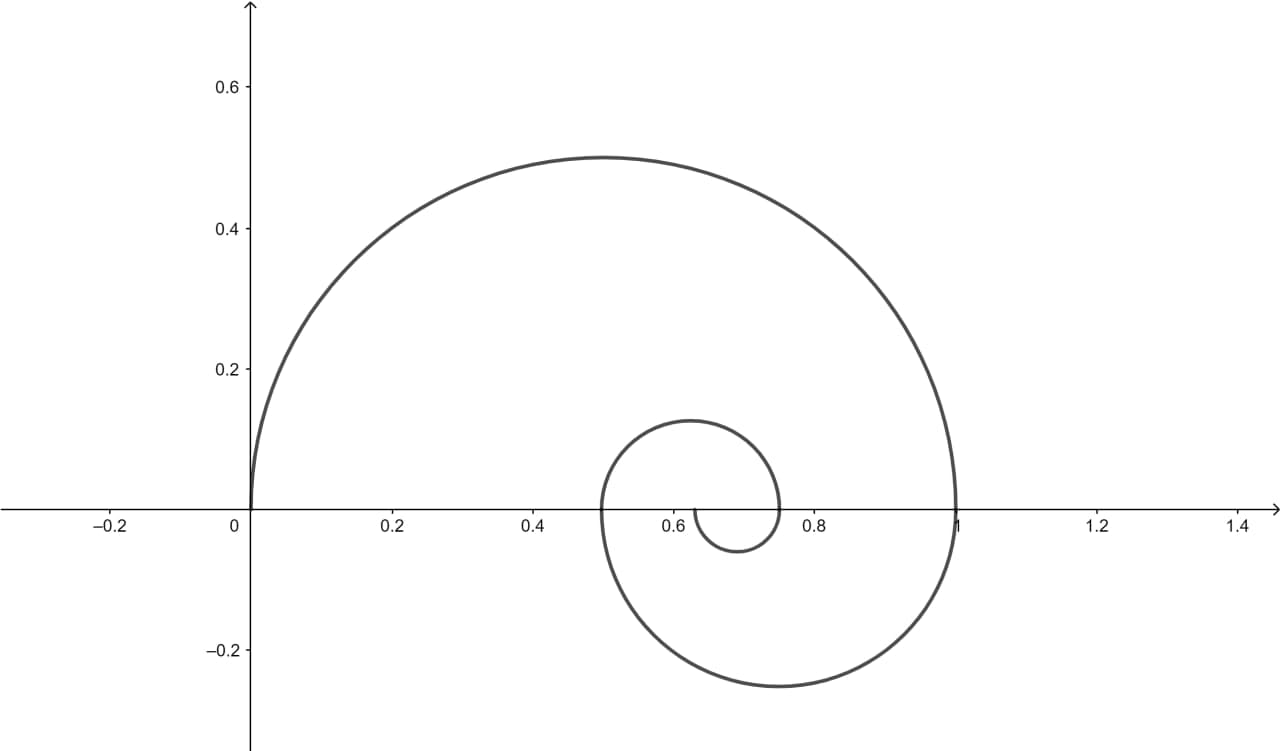
\includegraphics[width=15cm]{\imgdirfromsection/exercicio-espiral.png}
		\caption{Espiral de semicírculos.}
    \end{figure}
    \begin{enumerate}[a)]
        \item Se o diâmetro do primeiro semicírculo é igual a 1 e os seguintes são a metade do anterior, escreva uma PG $(d_1, d_2, d_3 , \dots)$, determinando razão e termo geral $d_n$, onde $d_n$ é a medida do diâmetro do $n$-ésimo semicírculo;
        \item Determine uma PG $(b_1, b_2, b_3 , \dots)$, incluindo razão e termo geral $b_n$, de tal forma que $b_1 = a_1$ e $b_i = a_i - a_{i-1}$ para todo $i \geq 2$;
        \item Calcule $a_n$ em função de $n$.
        \end{enumerate}
\end{exercise}

\begin{exercise}
    Uma \aspas{espiral} é montada em um quadriculado escrevendo os números naturais não nulos como na figura abaixo. Considere a sequência que aparece ao longo da seta com os números $(1, 3, 13, 31, \dots , a_n, \dots)$.
    \begin{figure}[H]
        \centering
        \label{fig:exercicio-espiral}
        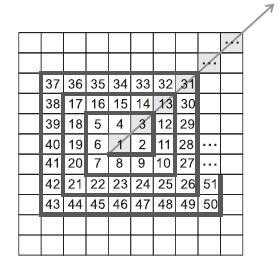
\includegraphics[width=7cm]{\imgdirfromsection/exercicio-espiral_de_numeros.png}
		\caption{Espiral de números.}
    \end{figure}
\begin{enumerate}[a)]
\item A sequência $(d_n)_{n \in \N^\ast}$, definida por $d_n = a_{n+1} - a_n$ para todo $n \in \N^\ast$, é uma PA. Determine essa PA indicando sua razão e seu termo geral.
\item Obtenha uma fórmula para $a_n$, com $n \in \N^\ast$.
\end{enumerate}
\end{exercise}

%EXERCÍCIOS PARA FUNÇÕES EXPONENCIAIS E LOGARÍTMICAS
%\Ex{Se $\paren{a_n}$ é uma PG de termos positivos, prove que
%$\paren{ b_n}$ definida por $b_n = \log a_n$ é uma PA.}

%\Ex{Se $\paren{a_n}$ é uma PA, prove que $\paren{ b_n}$ definida por
%$b_n = e^{a_n}$ é uma PG.}
